% To je predloga za poročila o domačih nalogah pri predmetih, katerih
% nosilec je Tomaž Curk. Avtor predloge je Blaž Zupan.
%
% Seveda lahko tudi dodaš kakšen nov, zanimiv in uporaben element,
% ki ga v tej predlogi (še) ni. Več o LaTeX-u izveš na
% spletu, na primer na http://tobi.oetiker.ch/lshort/lshort.pdf.%
% To predlogo lahko spremeniš v PDF dokument s pomočjo programa
% pdflatex, ki je del standardne instalacije LaTeX programov.

\documentclass[a4paper,11pt]{article}
\usepackage{a4wide}
\usepackage{fullpage}
\usepackage[utf8x]{inputenc}
\usepackage[english]{babel}
\selectlanguage{english}
\usepackage[toc,page]{appendix}
\usepackage[pdftex]{graphicx} % za slike
\usepackage{setspace}
\usepackage{color}
\definecolor{light-gray}{gray}{0.95}
\usepackage{listings}
\lstset{
  basicstyle=\ttfamily,
  columns=fullflexible,
  frame=single,
  breaklines=true,
  postbreak=\mbox{\textcolor{red}{$\hookrightarrow$}\space},
}
\usepackage{hyperref}
\renewcommand{\baselinestretch}{1.2} % za boljšo berljivost večji razmak
\renewcommand{\appendixpagename}{Appendix}

\lstset{ % nastavitve za izpis kode, sem lahko tudi kaj dodaš/spremeniš
language=Python,
basicstyle=\footnotesize,
basicstyle=\ttfamily\footnotesize\setstretch{1},
backgroundcolor=\color{light-gray},
}

\title{%
Analysis of song lyrics to match genre \\
\large Assignment 1: Basic text processing}
\author{Jernej Janež (63130077), Rok Marinšek (63130146), Luka Podgoršek (63130189)}
\date{\today}

\begin{document}

\maketitle

\section{NLP task}
% A paragraph of an NLP task/idea that you solved. A short description of your solution and related work in the field.
For our assignment we decided to analyze song lyrics, extract keywords that correspond to specific genres and try to classify song by its lyrics to corresponding genre. First we found a \href{https://www.kaggle.com/gyani95/380000-lyrics-from-metrolyrics}{\textit{dataset}} that contained song lyrics, then we preprocessed the data, trained and tested a model and presented results with tables and graphs. Some similar solutions already exist, but perform similar task with neural networks or some other more complex methods. With this assignment we wanted to find out if our approach can provide satisfactory results by using simple natural language processing techniques.

\section{Data}
% A description of (train, development, test) data or its retrieval
% Also describe metrics, used to score the performance of your algorithms.
We searched the internet for appropriate datasets and found many different ones but in the end decided to use \href{https://www.kaggle.com/gyani95/380000-lyrics-from-metrolyrics}{\textit{380,000+ lyrics from MetroLyrics dataset}} found on kaggle portal. This dataset had the attributes we needed to solve our task.

\noindent The dataset contained the following attributes:
\begin{itemize}
\item song title,
\item year,
\item artist
\item genre,
\item lyrics.
\end{itemize}

\subsection{Data preparation}
The data we found was stored in a \textit{.csv} file. Because it contained more than \textit{380 000} entries we decided to analyze songs that were released after year 2005 (latest songs in dataset). Afterwards we filtered the songs to match predefined genres which were \textit{hip-hop, pop and metal}. Then we removed songs with lyrics that had less than 100 words and more than 1000 words which removed the outliers in the data.

When we finished preparing and selecting the data we focused on text preparation. First we removed special characters from text with regular expressions, converted words to lowercase and removed punctuations. Finally we removed non-english songs. This way we ended up with \textbf{64605} different songs.

\begin{table}[h!]
\centering
\label{baseline}
\begin{tabular}{|clc|}
\hline
\# & Genre & Number of different songs \\
\hline
0 & Hip-Hop & 19574 \\
1 & Metal & 16187 \\
2 & Pop & 28844 \\
\hline
\end{tabular}
\caption{Number of songs per genre}
\end{table}

In the end we saved the filtered data into a \textit{.csv} file and used it as input in our model class to train our model. You can also use this file to replicate our results.

\section{Tools}

To build our model we used a preprocessed file and logistic regression.

\subsection{Train, test data and metrics}
% 80 20, regressing 0.2
% A description of (train, development, test) data or its retrieval. Also describe metrics, used to score the performance of your algorithms.
To train our model we used 80\% of data and 20\% to test our model. To measure score and performance of our model we used following metrics:
\begin{itemize}
\item accuracy,
\item precision,
\item recall,
\item and f1 score.
\end{itemize}

In development phase we also played with regularization factor. We used above mentioned metrics to determine the best regularization factor. In the end we set it to 0.1.

\subsection{Resources, tools and corpora}
%A description of tools and resources used. A list of additional linguistic corpora and how it was used to improve results of your algorithm

We used several different python libraries. Pandas was used for data structures and data purging. Nltk corpus was used to determine stopwords and for lemmatization. Langdetect library was used to remove non-english lyrics. To build our model we used sklearn and presented results with matplotlib.

\pagebreak
\section{Algorithm description}
% describe how we build our model

% we used l regression-.....

\subsection{Data feature extraction}
\label{feature-extraction}
Features were determined by the Bag-Of-Words approach using the data of column \textit{lyrics}.
Our tokenizer has three roles: tokenize words using whitespaces (NLTK's WhitespaceTokenizer), ignore stopwords and lemmatize each word.
Each extracted feature has a corresponding TF-IDF value (using sklearn's TfidfVectorizer).

\subsection{Model}
Our training data was constructed using the approach described in \ref{feature-extraction}.
To train our model for genre prediction we used sklearn's multinomial LogisticRegression classifer. 

To determine keywords for each genre we simply looked at the trained models weights and connected them to the corresponding feature.
We decided to show only the 10 most significant words with the highest positive and negative weights, thinking those words represent the genre best.

\section{Results}
% interpretacija modela, kaj je primerom skupno, zakaj pride do napačne klasifikacije

Before we could interpret our model and it's predictions we had to test it. Testing phase consisted of 10 iterations. In each iteration we sampled the data with different random seeds, trained a model and tested it on sampled test data. In the end we averaged all metrics to score the performance of our model. You can find the results in the \hyperref[label-model-score]{table} bellow.

\begin{table}[h!]
\centering
\label{baseline}
\begin{tabular}{|c|c|c|c|}
\hline
Accuracy & Precision & Recall & F1 \\
\hline
0.823 & 0.826 & 0.823 & 0.823 \\
\hline
\end{tabular}
\label{label-model-score}
\caption{Model scores}
\end{table}

\noindent Beside performance scores our model returned a list of keywords that have the most and the least value for classification. These results are presented in the tables bellow. Graphical presentation of tables is included in the appendix \hyperref[label-graphs]{graphs section.}

\begin{table}[h!]
\begin{tabular}{|lc|lc|}
\hline
(+) Keywords & Weight & (-) Keywords & Weight \\
\hline
death & 1.97 & love & -2.97 \\
blood & 1.88 & baby & -2.31 \\
dead & 1.85 & like & -2.29 \\
fucking & 1.65 & oh & -2.13 \\
pain & 1.57 & got & -1.98 \\
die & 1.56 & girl & -1.96 \\
end & 1.53 & i'm & -1.95 \\
lie & 1.46 & ain't & -1.81 \\
hate & 1.43 & yeah & -1.81 \\
fear & 1.43 & get & -1.64 \\
\hline
\end{tabular}
\quad
\begin{tabular}{|lc|lc|}
\hline
(+) Keywords & Weight & (-) Keywords & Weight \\
\hline
nigga & 3.71 & i've & -1.20 \\
shit & 2.71 & eye & -1.09 \\
yo & 2.48 & lie & -1.02 \\
ain't & 2.46 & dream & -0.94 \\
like & 2.38 & alone & -0.77 \\
bitch & 2.25 & inside & -0.77 \\
girl & 1.76 & heart & -0.77 \\
ya & 1.75 & end & -0.76 \\
cause & 1.69 & there's & -0.75 \\
got & 1.67 & away & -0.75 \\
\hline
\end{tabular}
\caption{Keywords for: \textbf{metal} (left) \& \textbf{hip-hop} (right)}
\end{table}

\begin{table}[h!]
\centering
\label{baseline}
\begin{tabular}{|lc|lc|}
\hline
(+) Keywords & Weight & (-) Keywords & Weight \\
\hline
love & 2.29 & nigga & -2.45 \\
oh & 1.93 & shit & -2.41 \\
heart & 1.56 & fuck & -2.14 \\
gonna & 1.29 & death & -1.76 \\
boy & 1.22 & fucking & -1.66 \\
baby & 1.16 & dead & -1.61 \\
'cause & 1.10 & die & -1.57 \\
could & 1.01 & bitch & -1.55 \\
there's & 0.97 & blood & -1.43 \\
kiss & 0.97 & hate & -1.37 \\
\hline
\end{tabular}
\caption{Keywords for \textbf{pop}}
\end{table}

\subsection{POS tagging}
%top nouns and adjectives per genre

To gain further insight into our model's keywords we decided to POS tag them.
We extracted the 10 most (+) significant nouns, adjectives and verbs for each genre.
The resulting words are visible in the tables \hyperref[label-hip-hop-pos]{5}, \hyperref[label-metal-pos]{6} and \hyperref[label-pop-pos]{7} below.
We find the results not to be surprising, especially the nouns are something that should be recognizable to each fan of the genres (and also confirm certain stereotypes we have about the genres).

\begin{table}[h!]
\centering
\begin{tabular}{|l|c|}
\hline
Top verbs & Weight \\
\hline
got & 1.67 \\
get & 1.67 \\
keep & 0.68 \\
go & 0.62 \\
hundred & 0.57 \\
said & 0.54 \\
know & 0.54 \\
started & 0.45 \\
came & 0.44 \\
slow & 0.41 \\
\hline
\end{tabular}
\quad
\begin{tabular}{|l|c|}
\hline
Top nouns & Weight \\
\hline
nigga & 3.71 \\
shit & 2.71 \\
yo & 2.48 \\
ain't & 2.46 \\
bitch & 2.25 \\
girl & 1.76 \\
ya & 1.75 \\
cause & 1.69 \\
'em & 1.66 \\
i'm & 1.66 \\
\hline
\end{tabular}
\quad
\begin{tabular}{|l|c|}
\hline
Top adjectives & Weight \\
\hline
whole & 0.91 \\
big & 0.82 \\
real & 0.79 \\
black & 0.60 \\
fresh & 0.49 \\
high & 0.48 \\
low & 0.48 \\
nice & 0.45 \\
next & 0.42 \\
new & 0.41 \\
\hline
\end{tabular}
\caption{Hip-hop POS tagging}
\label{label-hip-hop-pos}
\end{table}


\begin{table}[h!]
\centering
\begin{tabular}{|l|c|}
\hline
Top verbs & Weight \\
\hline
fucking & 1.65 \\
dying & 0.83 \\
hatred & 0.67 \\
lost & 0.66 \\
forced & 0.60 \\
suffering & 0.58 \\
killing & 0.57 \\
damned & 0.56 \\
wing & 0.51 \\
screaming & 0.50 \\
\hline
\end{tabular}
\quad
\begin{tabular}{|l|c|}
\hline
Top nouns & Weight \\
\hline
death & 1.97 \\
blood & 1.88 \\
pain & 1.57 \\
die & 1.56 \\
end & 1.53 \\
lie & 1.46 \\
hate & 1.43 \\
fear & 1.43 \\
soul & 1.36 \\
hell & 1.30 \\
\hline
\end{tabular}
\quad
\begin{tabular}{|l|c|}
\hline
Top adjectives & Weight \\
\hline
dead & 1.85 \\
final & 1.14 \\
eternal & 0.91 \\
alive & 0.69 \\
black & 0.61 \\
empty & 0.54 \\
unknown & 0.51 \\
false & 0.50 \\
free & 0.49 \\
last & 0.48 \\
\hline
\end{tabular}
\caption{Metal POS tagging}
\label{label-metal-pos}
\end{table}


\begin{table}[h!]
\centering
\begin{tabular}{|l|c|}
\hline
Top verbs & Weight \\
\hline
know & 0.90 \\
say & 0.80 \\
loving & 0.73 \\
darling & 0.68 \\
find & 0.63 \\
feeling & 0.61 \\
believe & 0.59 \\
go & 0.58 \\
let & 0.56 \\
dancing & 0.55 \\
\hline
\end{tabular}
\quad
\begin{tabular}{|l|c|}
\hline
Top nouns & Weight \\
\hline
love & 2.29 \\
oh & 1.93 \\
heart & 1.56 \\
gonna & 1.29 \\
boy & 1.22 \\
baby & 1.16 \\
'cause & 1.10 \\
there's & 0.97 \\
kiss & 0.97 \\
ooh & 0.96 \\
\hline
\end{tabular}
\quad
\begin{tabular}{|l|c|}
\hline
Top adjectives & Weight \\
\hline
little & 0.76 \\
easy & 0.53 \\
happy & 0.51 \\
good & 0.45 \\
small & 0.39 \\
lucky & 0.32 \\
much & 0.28 \\
tiny & 0.26 \\
old & 0.24 \\
impossible & 0.23 \\
\hline
\end{tabular}
\caption{Pop POS tagging}
\label{label-pop-pos}
\end{table}

\pagebreak
% slabosti modela
\subsection{Understanding wrong classifications}

If you look at our \hyperref[label-cf-matrix]{confusion matrix} you can notice that most commonly miss-classified songs are pop songs. We didn't expect to classify every song correctly, but pop songs have larger error rate than metal or hip-hop songs. We tried to understand why this was happening and our hypothesis was that many pop song artists feature artists from hip-hop or metal and therefore correlate with actual hip-hop and metal songs.


\section{Conclusion}

When we tested our hypothesis we found one particular interesting example. Song \href{https://www.youtube.com/watch?v=iKFYrPH5nRI}{The Reckoning from Blood On The Dance Floor} was classified as metal. In dataset this song is represented as pop song. We listened to the song and realized that the lyrics were consistent with metal lyrics. That's why our model predicted this song as metal instead of pop. This example shows us that some songs are about similar topics but correspond to different genre.

Besides that we found out that the dataset was not perfect. Some songs didn't have correct genre listed. For example, Swedish metal band Bewitched is stored in dataset as pop. These kind of errors in dataset influenced our model and end results.

We believe that you can predict to some extent in which genre song belongs by analyzing song lyrics. But this approach is a bit flawed. If you want to predict genre with high degree of certainty you need to add some other techniques like analyzing sound.


\section{Github repository}
Github repository: \href{https://github.com/marok39/onj-02}{https://github.com/marok39/onj-02}

\pagebreak
\appendix
\appendixpage
\section{\label{label-graphs} Graphs}

Here you can find the visualization of all results. These files can be found alongside the report in \textit{/img} directory.

\begin{figure}[h]
\begin{center}
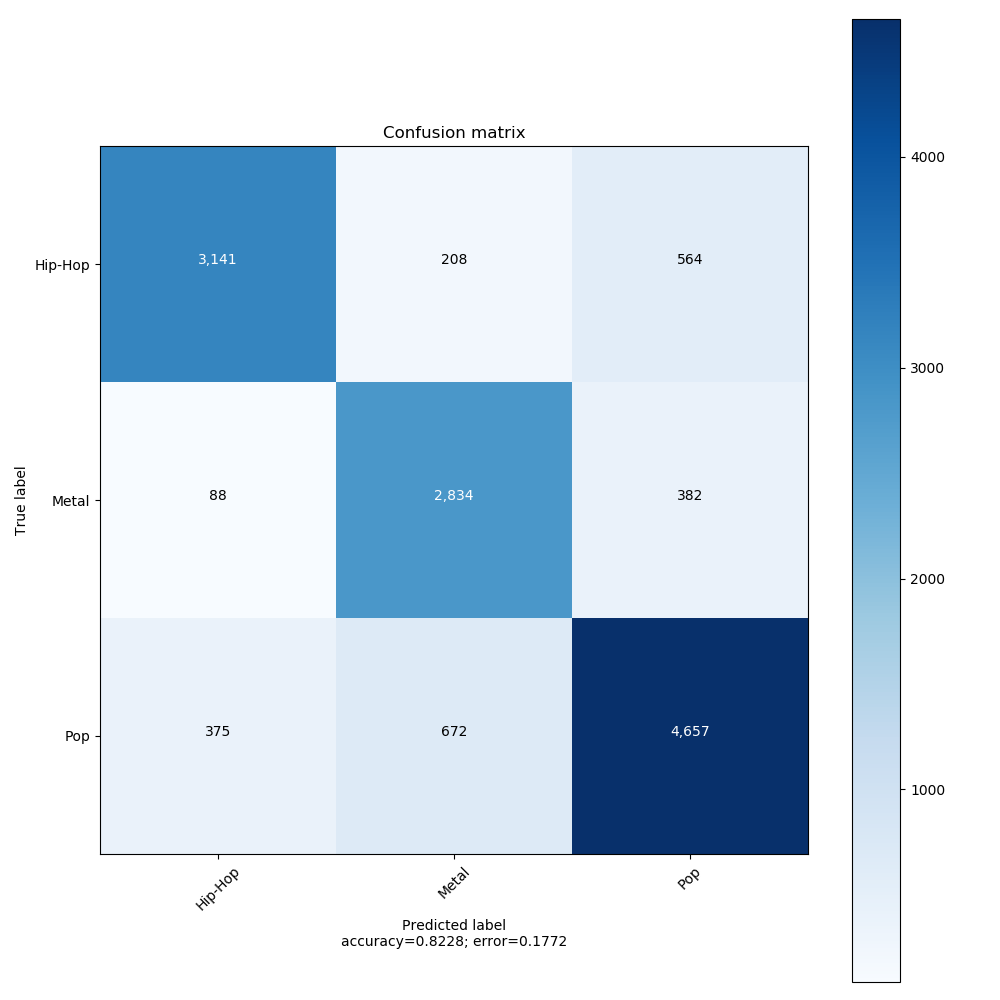
\includegraphics[width=0.8\textwidth]{./img/matrix.png}
\end{center}
\caption{Confusion matrix}
\label{label-cf-matrix}
\end{figure}

\begin{figure}[h]
\begin{center}
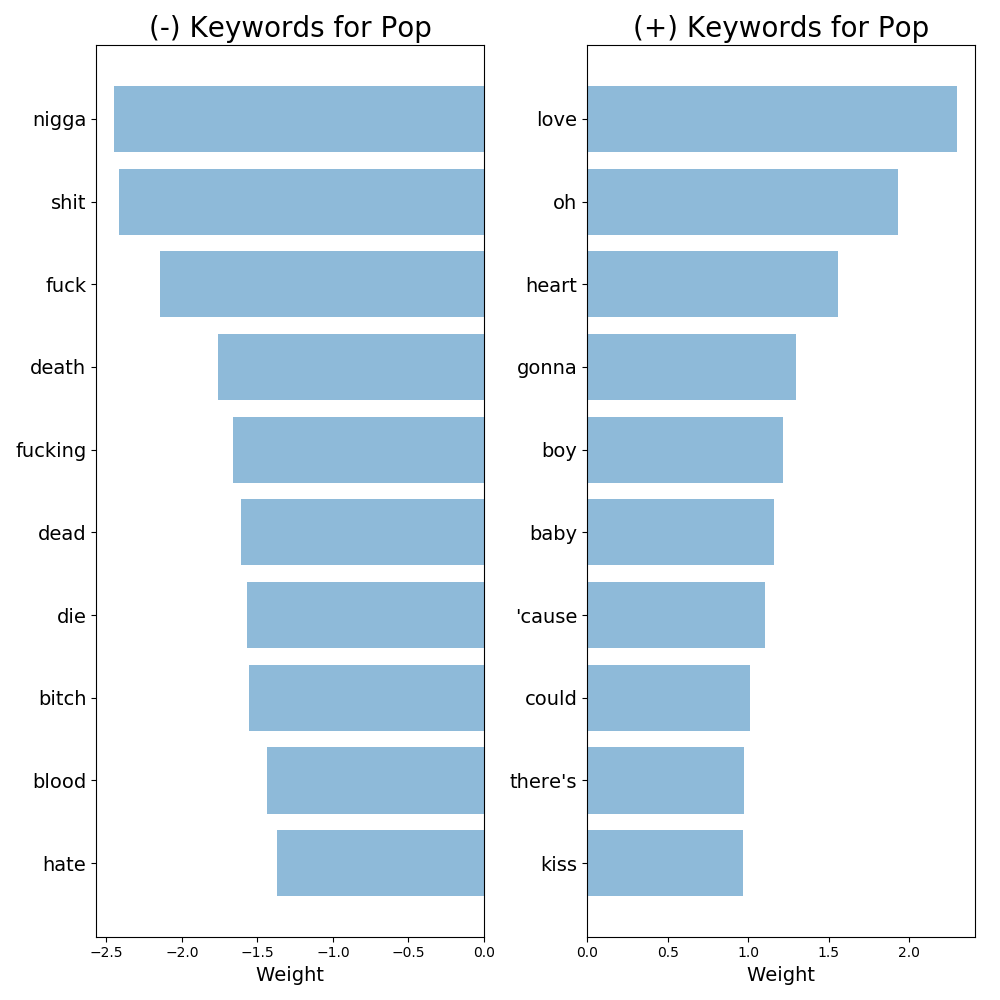
\includegraphics[width=0.8\textwidth]{./img/pop-keywords.png}
\end{center}
\caption{Keywords visualization for pop}
\label{label-kw-pop}
\end{figure}

\begin{figure}[h]
\begin{center}
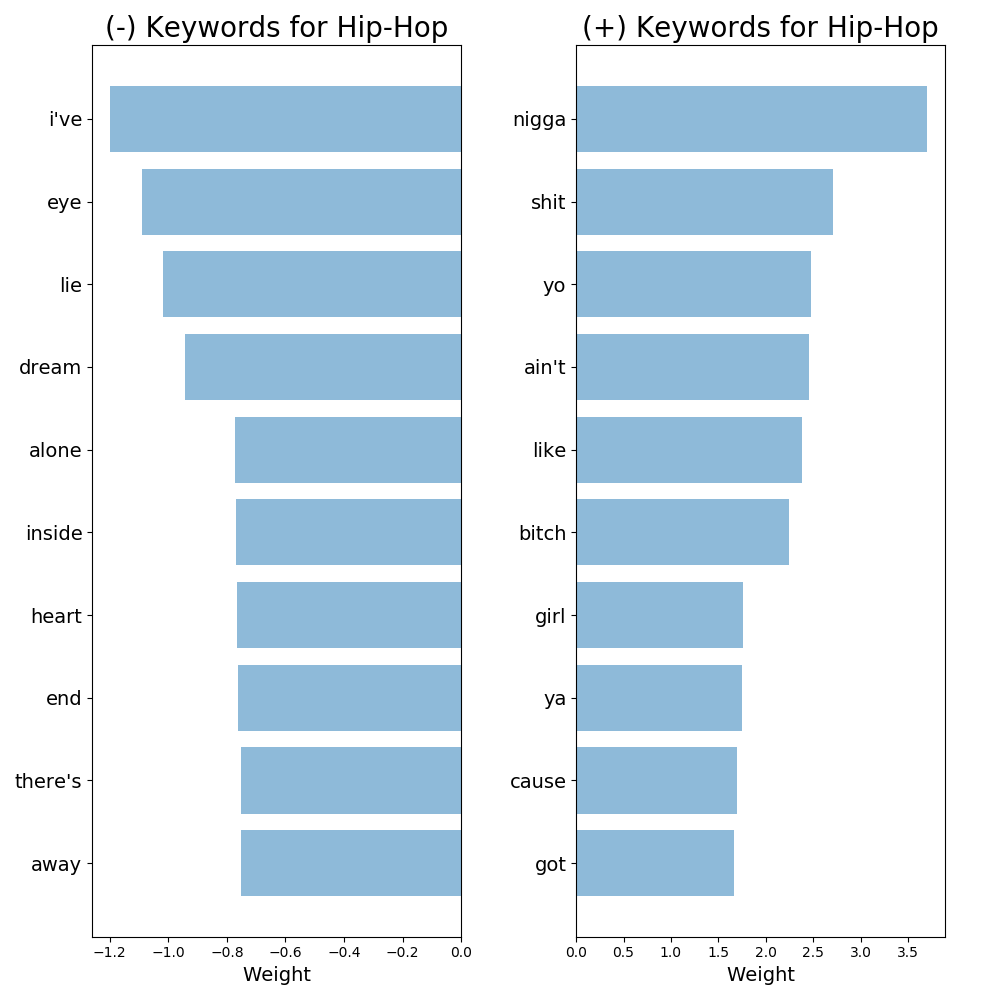
\includegraphics[width=0.8\textwidth]{./img/hip-hop-keywords.png}
\end{center}
\caption{Keywords visualization for hip-hop}
\label{label-kw-hip-hop}
\end{figure}

\begin{figure}[h]
\begin{center}
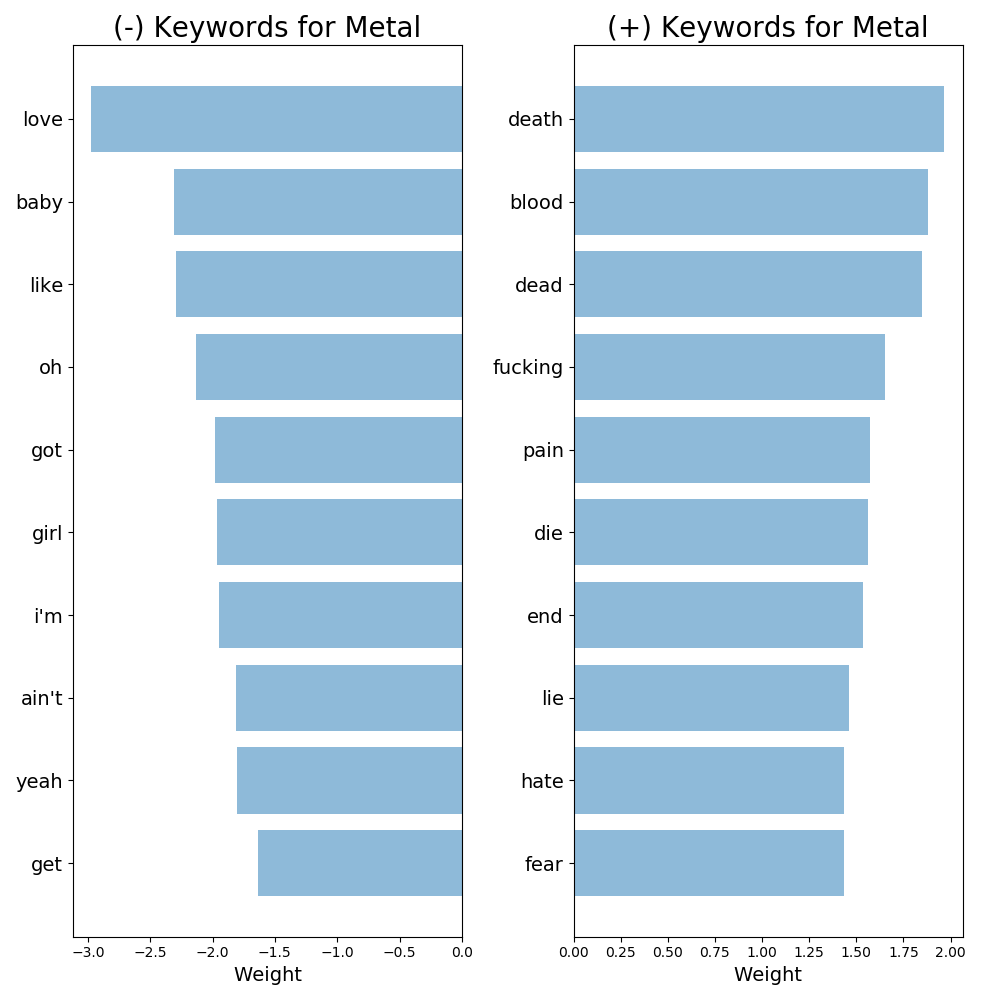
\includegraphics[width=0.8\textwidth]{./img/metal-keywords.png}
\end{center}
\caption{Keywords visualization for metal}
\label{label-kw-metal}
\end{figure}

%\begin{lstlisting}
%# comment
%\end{lstlisting}


\end{document}
